\begin{frame}{Resultado de MIX}
  $S$ ha sido el resultado de usar MIX, entonces nos retorna la siguiente gráfica

  \begin{figure}  
    \centering
    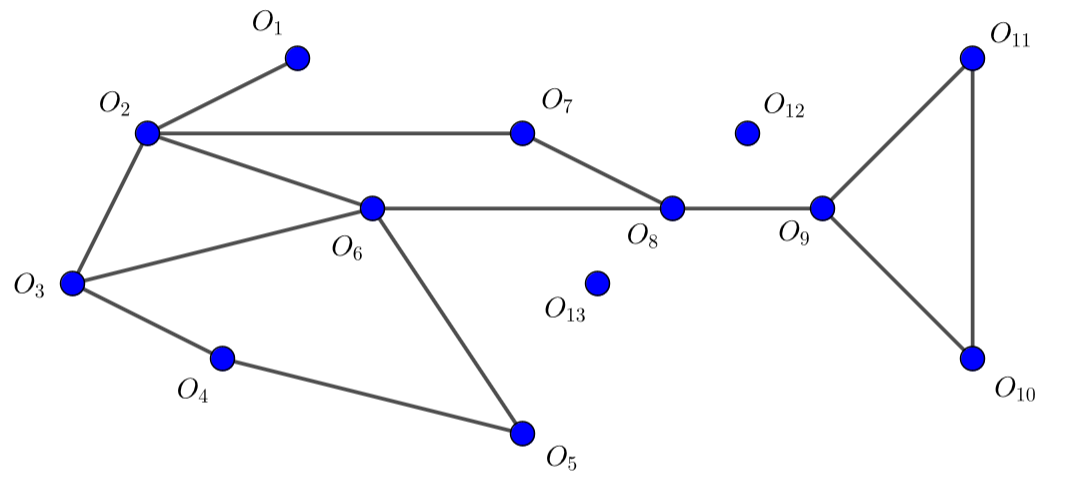
\includegraphics[width=1\textwidth]{./Images/ED01.png}
  \end{figure}
\end{frame}

\begin{frame}{Proyecciones en $\ell$-eje}
  Realicemos las proyecciones correspondientes en $X$

  \begin{figure}  
    \centering
    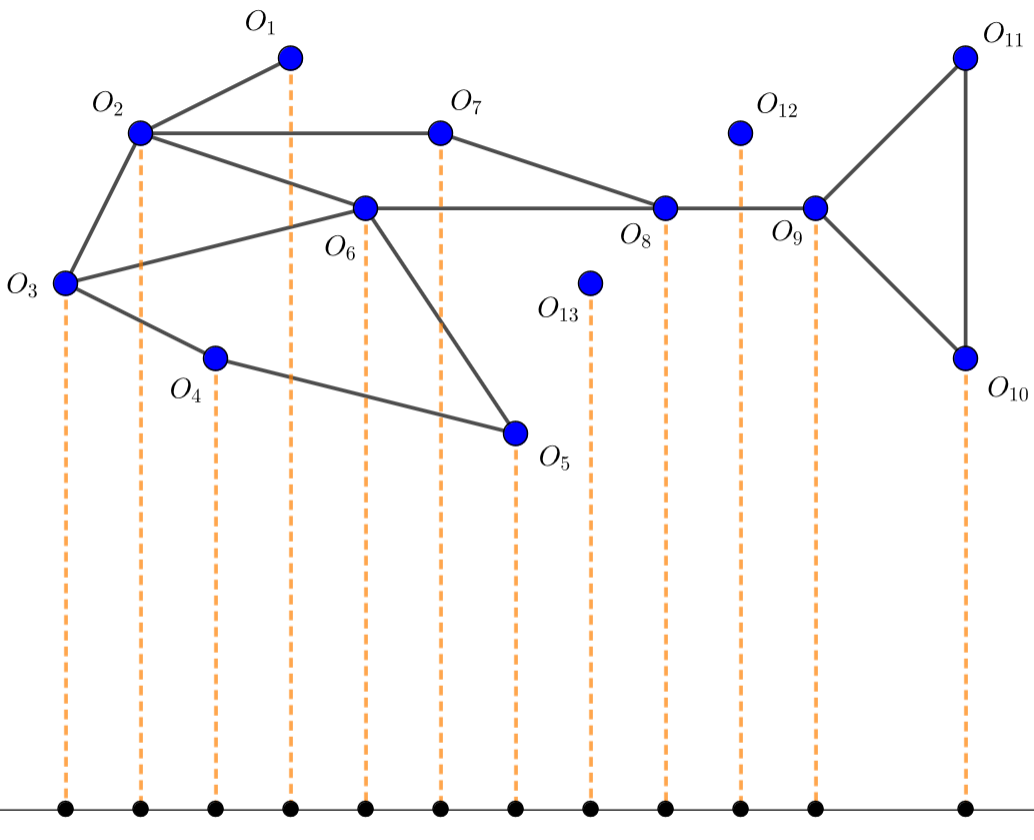
\includegraphics[width=0.8\textwidth]{./Images/ED02.png}
  \end{figure}
\end{frame}

\begin{frame}{Construcción del árbol de rangos}
  A continuación realizamos la construcción de un árbol de rangos

  \begin{figure}  
    \centering
    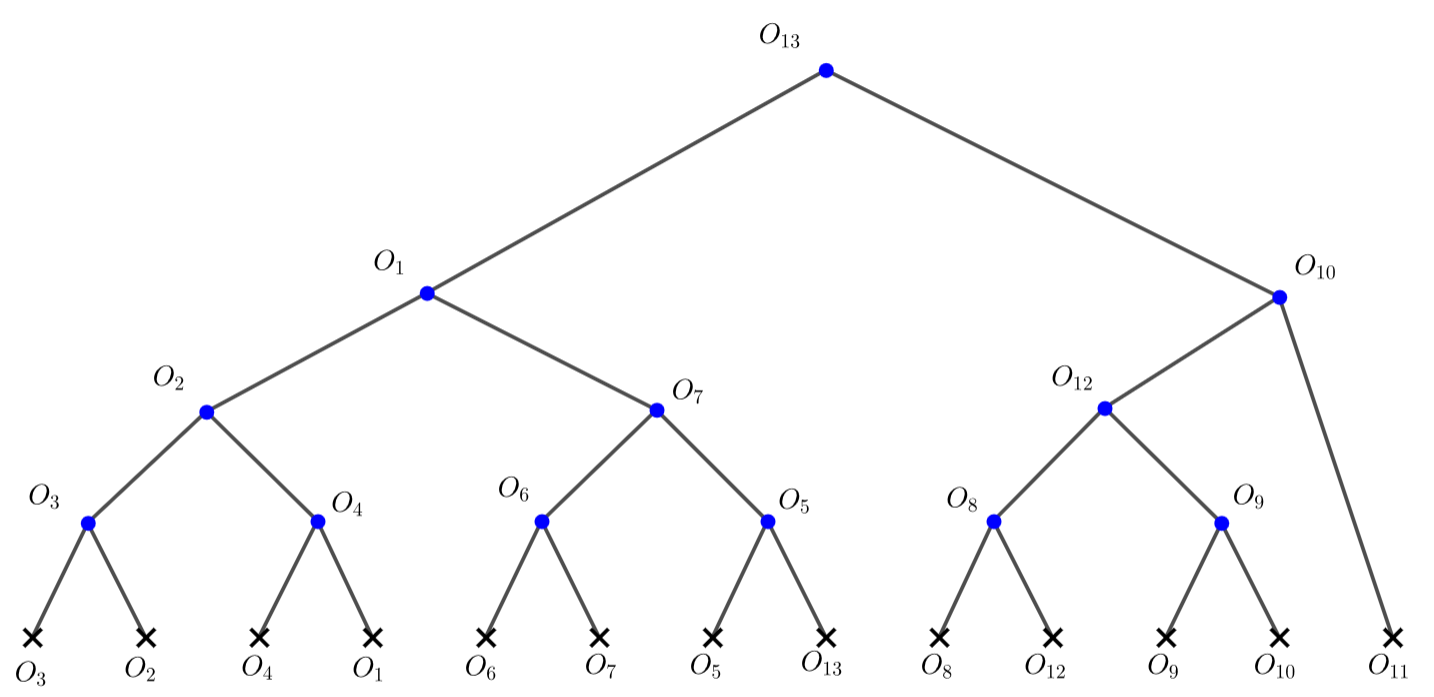
\includegraphics[width=1\textwidth]{./Images/Range1.png}
  \end{figure}
\end{frame}


\begin{frame}{...}
  Sea $T_1$ el árbol asociado a los discos en $S_1$

  \begin{figure}  
    \centering
    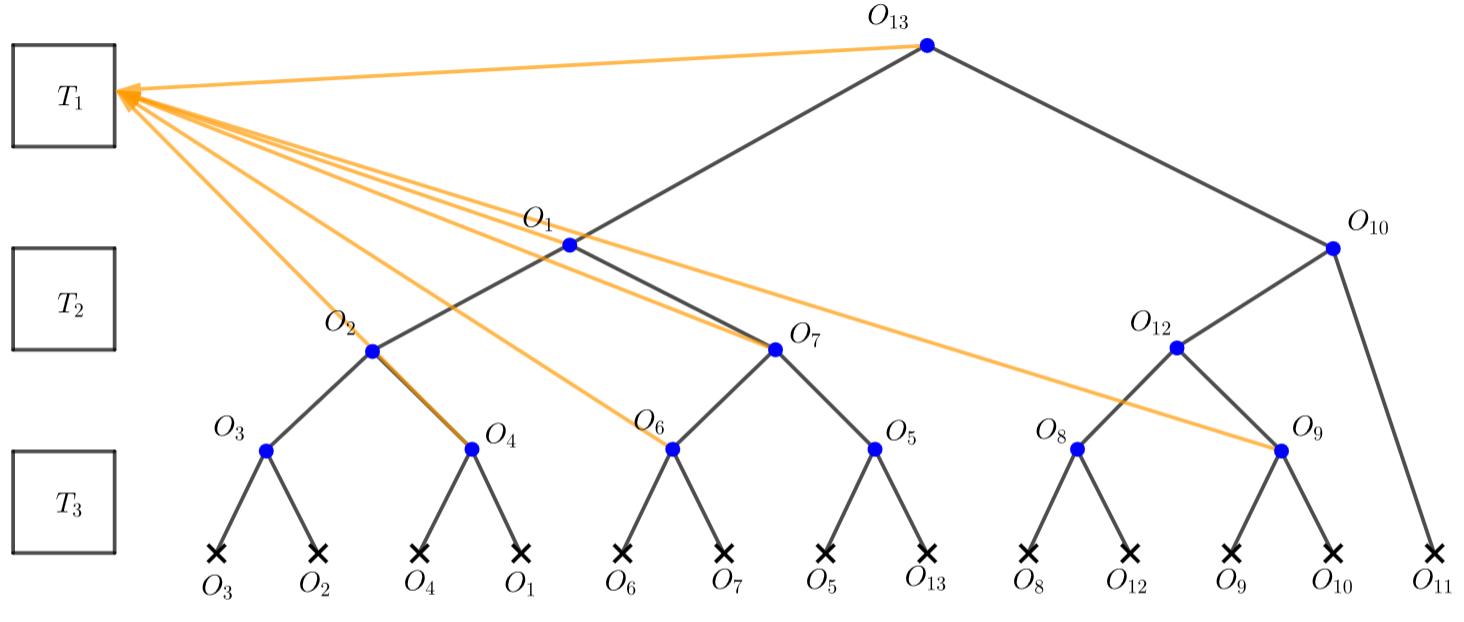
\includegraphics[width=1\textwidth]{./Images/Range2.png}
  \end{figure}
\end{frame}

\begin{frame}{...}
  Sea $T_2$ el árbol asociado a los discos en $S_2$

  \begin{figure}  
    \centering
    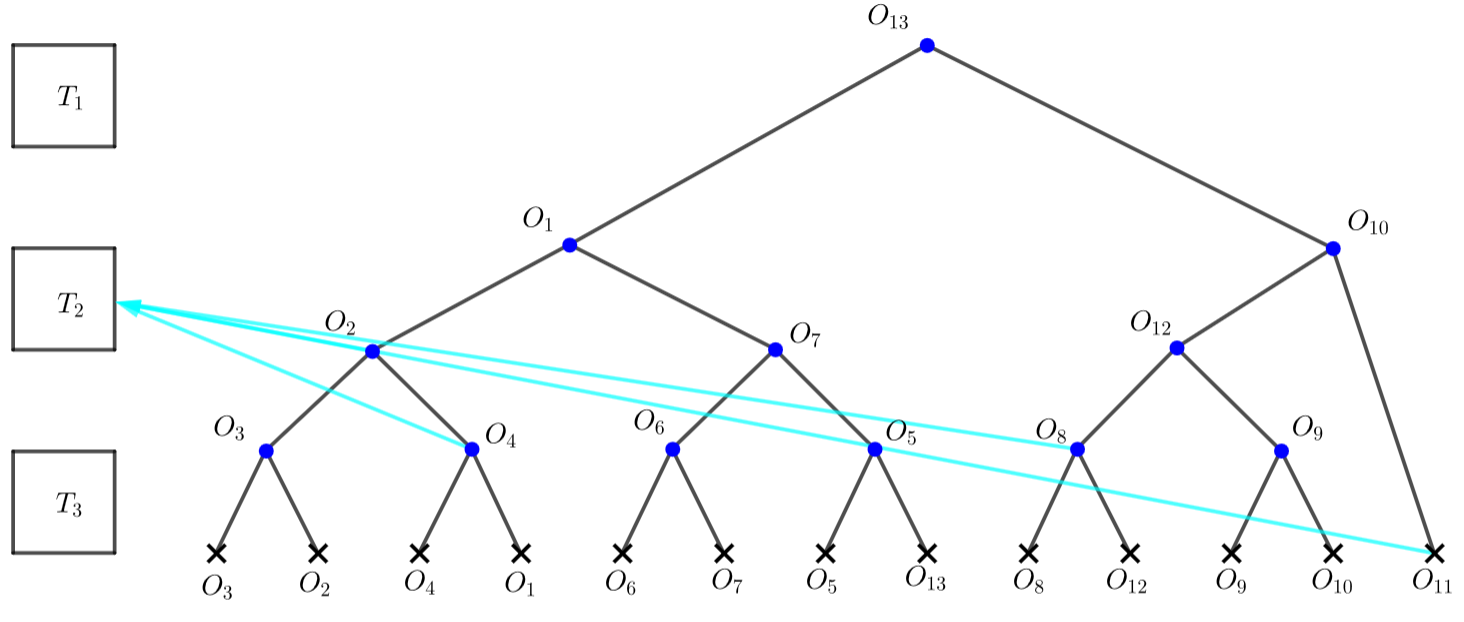
\includegraphics[width=1\textwidth]{./Images/Range3.png}
  \end{figure}
\end{frame}

\begin{frame}{...}
  Sea $T_3$ el árbol asociado a los discos en $S_3$

  \begin{figure}  
    \centering
    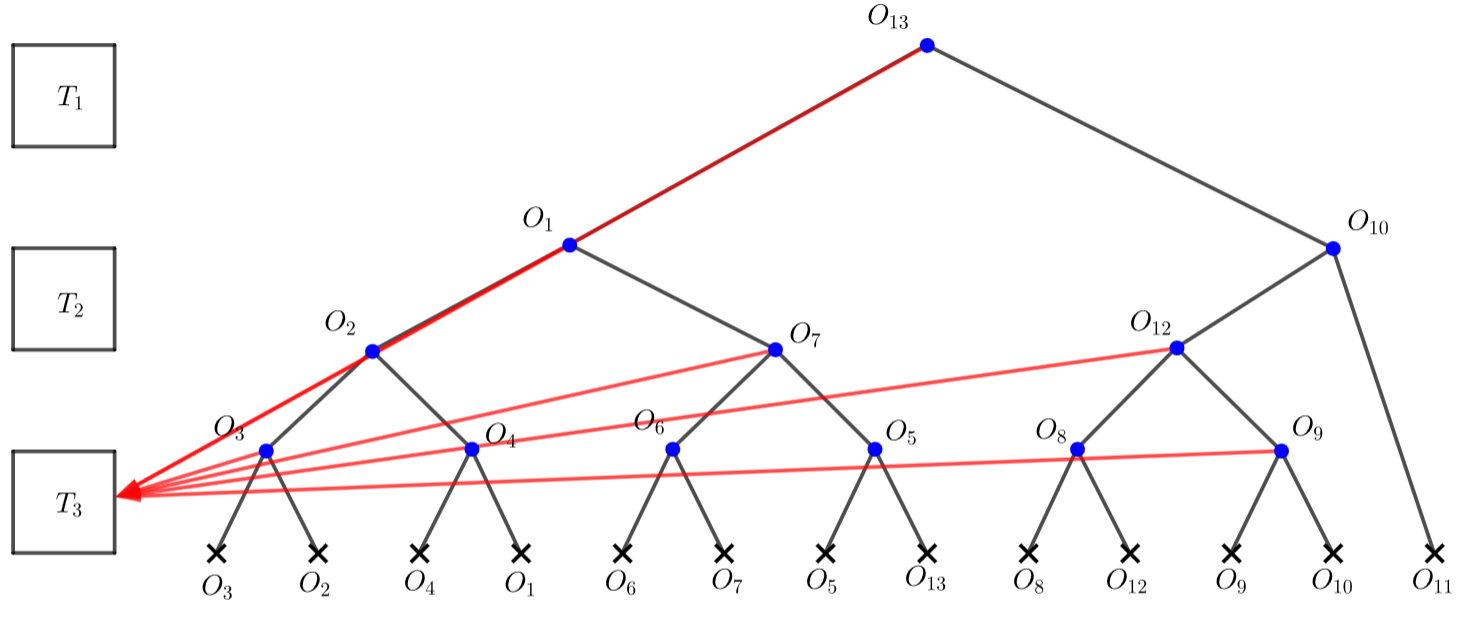
\includegraphics[width=1\textwidth]{./Images/Range4.png}
  \end{figure}
\end{frame}


\begin{frame}
  Comentarios sobre generalizaciones ...
\end{frame}
